% Fig. 1: the uranium and thorium decay series and the single nuclides measured, with the gamma lines used (keV).
% Half-lives and gamma energies from NuDat 3 (ENSDF), rounded.
\documentclass[11pt,border=4pt]{standalone}
\usepackage[T1]{fontenc}
\usepackage{newtxtext}
\usepackage{amsmath}
\usepackage{newtxmath}
\usepackage{xcolor}
\usepackage{siunitx}
\usepackage{tikz}
\usetikzlibrary{arrows.meta,positioning,calc}
\newcommand{\nuc}[2]{\textsuperscript{#1}#2}
\newcommand{\seetag}[1]{\par\vspace{2pt}\hfill{\setlength{\fboxsep}{1.5pt}\fcolorbox{blue!45!black}{white}{\textcolor{blue!45!black}{see #1}}}}
\begin{document}
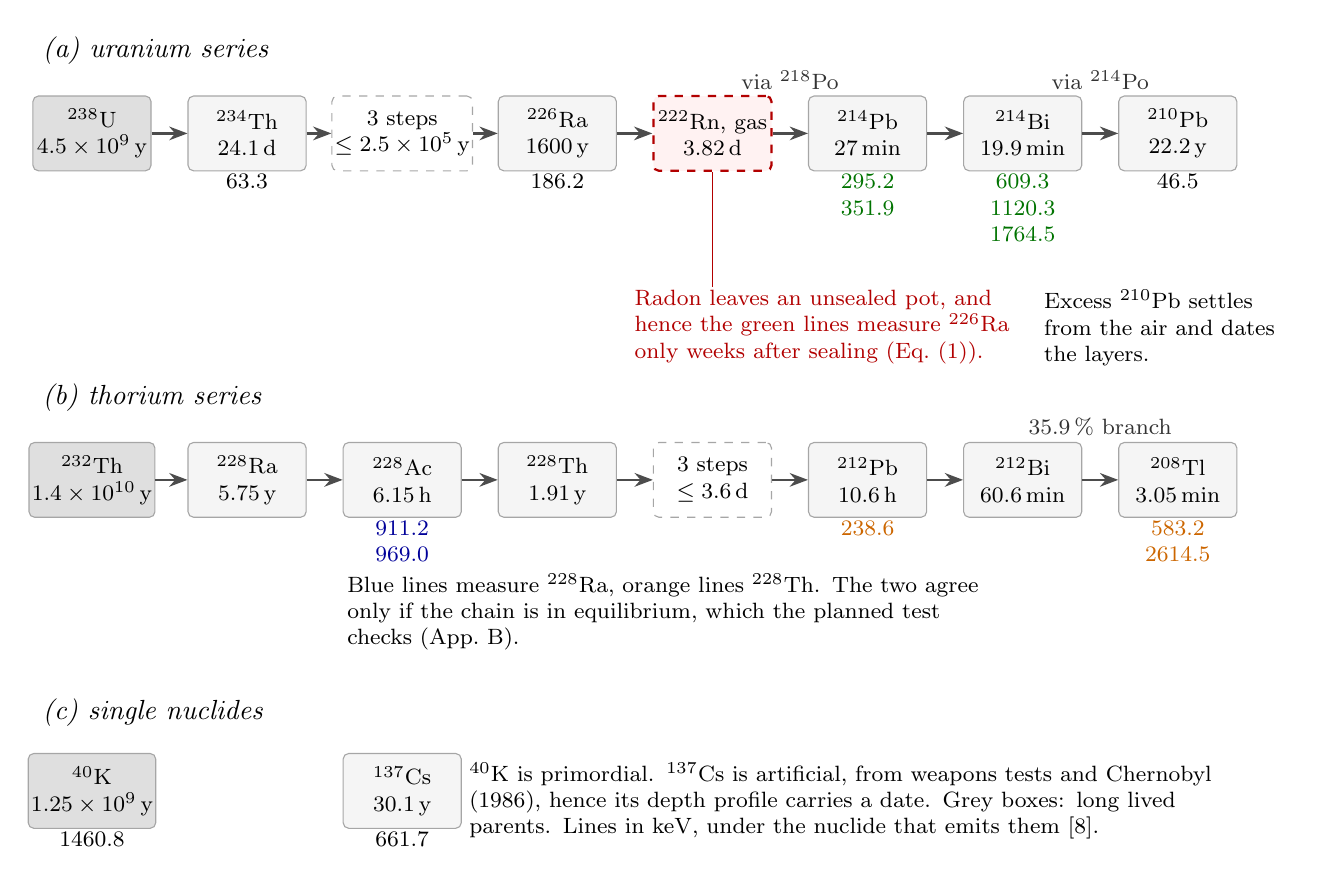
\begin{tikzpicture}[font=\footnotesize, >=Stealth,
  cnuc/.style={draw=gray!70, rounded corners=2pt, fill=gray!8, align=center, minimum width=1.5cm, minimum height=0.95cm, inner sep=1pt},
  cpar/.style={cnuc, fill=gray!25},
  cgas/.style={cnuc, draw=red!70!black, dashed, thick, fill=red!5},
  cgrp/.style={cnuc, fill=white, dashed},
  clin/.style={align=center, anchor=north, inner sep=1pt},
  cch/.style={->, thick, gray!60!black},
  cnote/.style={align=left, anchor=north west, text width=4.9cm, inner sep=1pt}]
\def\dx{1.97}
% ------------------------------------------------------------ uranium series
\node[anchor=west, font=\normalsize\itshape] at (-0.75,1.05) {(a) uranium series};
\node[cpar] (u0) at (0*\dx,0) {{\nuc{238}{U}}\\$4.5\times10^{9}$\,y};
\node[cnuc] (u1) at (1*\dx,0) {{\nuc{234}{Th}}\\24.1\,d};
\node[cgrp] (u2) at (2*\dx,0) {3 steps\\$\le 2.5\times10^{5}$\,y};
\node[cnuc] (u3) at (3*\dx,0) {{\nuc{226}{Ra}}\\1600\,y};
\node[cgas] (u4) at (4*\dx,0) {{\nuc{222}{Rn}}, gas\\3.82\,d};
\node[cnuc] (u5) at (5*\dx,0) {{\nuc{214}{Pb}}\\27\,min};
\node[cnuc] (u6) at (6*\dx,0) {{\nuc{214}{Bi}}\\19.9\,min};
\node[cnuc] (u7) at (7*\dx,0) {{\nuc{210}{Pb}}\\22.2\,y};
\foreach \a/\b in {u0/u1,u1/u2,u2/u3,u3/u4,u5/u6} \draw[cch] (\a) -- (\b);
\draw[cch] (u4) -- node[above=6pt, inner sep=1pt, font=\scriptsize] {} (u5);
\draw[cch] (u6) -- (u7);
\node[font=\footnotesize, gray!40!black] at ($(u4)!0.5!(u5)+(0,0.68)$) {via {{\nuc{218}{Po}}}};
\node[font=\footnotesize, gray!40!black] at ($(u6)!0.5!(u7)+(0,0.68)$) {via {{\nuc{214}{Po}}}};
\node[clin] at (u1.south) {63.3};
\node[clin] at (u3.south) {186.2};
\node[clin, green!45!black] at (u5.south) {295.2\\351.9};
\node[clin, green!45!black] at (u6.south) {609.3\\1120.3\\1764.5};
\node[clin] at (u7.south) {46.5};
\node[cnote, red!70!black] at (6.85,-1.95) {Radon leaves an unsealed pot, and hence the green lines measure {{\nuc{226}{Ra}}} only weeks after sealing (Eq.~(1)).};
\node[cnote, text width=3.1cm] at (12.05,-1.95) {Excess {{\nuc{210}{Pb}}} settles from the air and dates the layers.};
\draw[red!70!black, thin] (u4.south) -- (7.88,-1.95);
% ------------------------------------------------------------ thorium series
\node[anchor=west, font=\normalsize\itshape] at (-0.75,-3.35) {(b) thorium series};
\node[cpar] (t0) at (0*\dx,-4.4) {{\nuc{232}{Th}}\\$1.4\times10^{10}$\,y};
\node[cnuc] (t1) at (1*\dx,-4.4) {{\nuc{228}{Ra}}\\5.75\,y};
\node[cnuc] (t2) at (2*\dx,-4.4) {{\nuc{228}{Ac}}\\6.15\,h};
\node[cnuc] (t3) at (3*\dx,-4.4) {{\nuc{228}{Th}}\\1.91\,y};
\node[cgrp] (t4) at (4*\dx,-4.4) {3 steps\\$\le 3.6$\,d};
\node[cnuc] (t5) at (5*\dx,-4.4) {{\nuc{212}{Pb}}\\10.6\,h};
\node[cnuc] (t6) at (6*\dx,-4.4) {{\nuc{212}{Bi}}\\60.6\,min};
\node[cnuc] (t7) at (7*\dx,-4.4) {{\nuc{208}{Tl}}\\3.05\,min};
\foreach \a/\b in {t0/t1,t1/t2,t2/t3,t3/t4,t4/t5,t5/t6} \draw[cch] (\a) -- (\b);
\draw[cch] (t6) -- (t7);
\node[font=\footnotesize, gray!40!black] at ($(t6)!0.5!(t7)+(0,0.68)$) {35.9\,\% branch};
\node[clin, blue!60!black] at (t2.south) {911.2\\969.0};
\node[clin, orange!80!black] at (t5.south) {238.6};
\node[clin, orange!80!black] at (t7.south) {583.2\\2614.5};
\node[cnote, text width=8.2cm] at (3.2,-5.55) {Blue lines measure {{\nuc{228}{Ra}}}, orange lines {{\nuc{228}{Th}}}. The two agree only if the chain is in equilibrium, which the planned test checks (App.~B).};
% ------------------------------------------------------------ single nuclides
\node[anchor=west, font=\normalsize\itshape] at (-0.75,-7.35) {(c) single nuclides};
\node[cpar] (k) at (0*\dx,-8.35) {{\nuc{40}{K}}\\$1.25\times10^{9}$\,y};
\node[clin] at (k.south) {1460.8};
\node[cnuc] (c) at (2*\dx,-8.35) {{\nuc{137}{Cs}}\\30.1\,y};
\node[clin] at (c.south) {661.7};
\node[cnote, text width=9.6cm] at (4.75,-7.95) {{\nuc{40}{K}} is primordial. {{\nuc{137}{Cs}}} is artificial, from weapons tests and Chernobyl (1986), hence its depth profile carries a date. Grey boxes: long lived parents. Lines in keV, under the nuclide that emits them~[8].};
\end{tikzpicture}
\end{document}
